\documentclass[11pt, addpoints]{exam}

\bibliographystyle{abbrv}

\usepackage{amsfonts}

\usepackage{amsthm}

\usepackage{amssymb}

\usepackage{amsmath}

\usepackage{enumerate}

\usepackage[all]{xy}

\usepackage{graphicx}

\usepackage{tikz}

\usepackage{pgfplots}

\usetikzlibrary{arrows}

\newcommand{\N}{\mathbb{N}}

\newcommand{\Z}{\mathbb{Z}}

\newcommand{\R}{\mathbb{R}}

\newcommand{\Q}{\mathbb{Q}}

\newcommand{\C}{\mathbb{C}}

\newcommand{\T}{\mathbb{T}}

\newcommand{\ra}{~~\Rightarrow~~}

\newcommand{\lra}{~~\Leftrightarrow~~}

\setlength{\unitlength}{1.5cm}

\addpoints

\begin{document}




\section*{Math 241 Summer 2023 Final}

\textbf{Name:}

\begin{flushright}
\gradetable[v][questions]
\end{flushright}     

\begin{itemize}
\item You may not use calculators on the test.  
\item You may use \textbf{paper} notes on the test.
\item Please ask if anything seems confusing or ambiguous.
\item You must show all your work and make clear what your final solution is (e.g.\ by drawing a box around it).
\item Good luck!
\end{itemize}

           

\pagebreak

[This page is intentionally left almost blank.]

\pagebreak

\begin{questions}

\question[40] Sketch the curve $f(x)$ given by
\[f(x) = \frac{x^2-1}{x^3}.\]
Find the following values exactly:
\begin{itemize}
    \item Roots of $f$.
    \item Vertical and horizontal asymptotes of $f$.
    \item Intervals of increase and decrease.
    \item Absolute minimums and absolute maximums, if they exist.
    \item Local minimums and local maximums, if they exist.
    \item Intervals of concavity.
    \item Inflection points, if they exist.
\end{itemize}
\pagebreak
$\ $
\vfill
\begin{center}
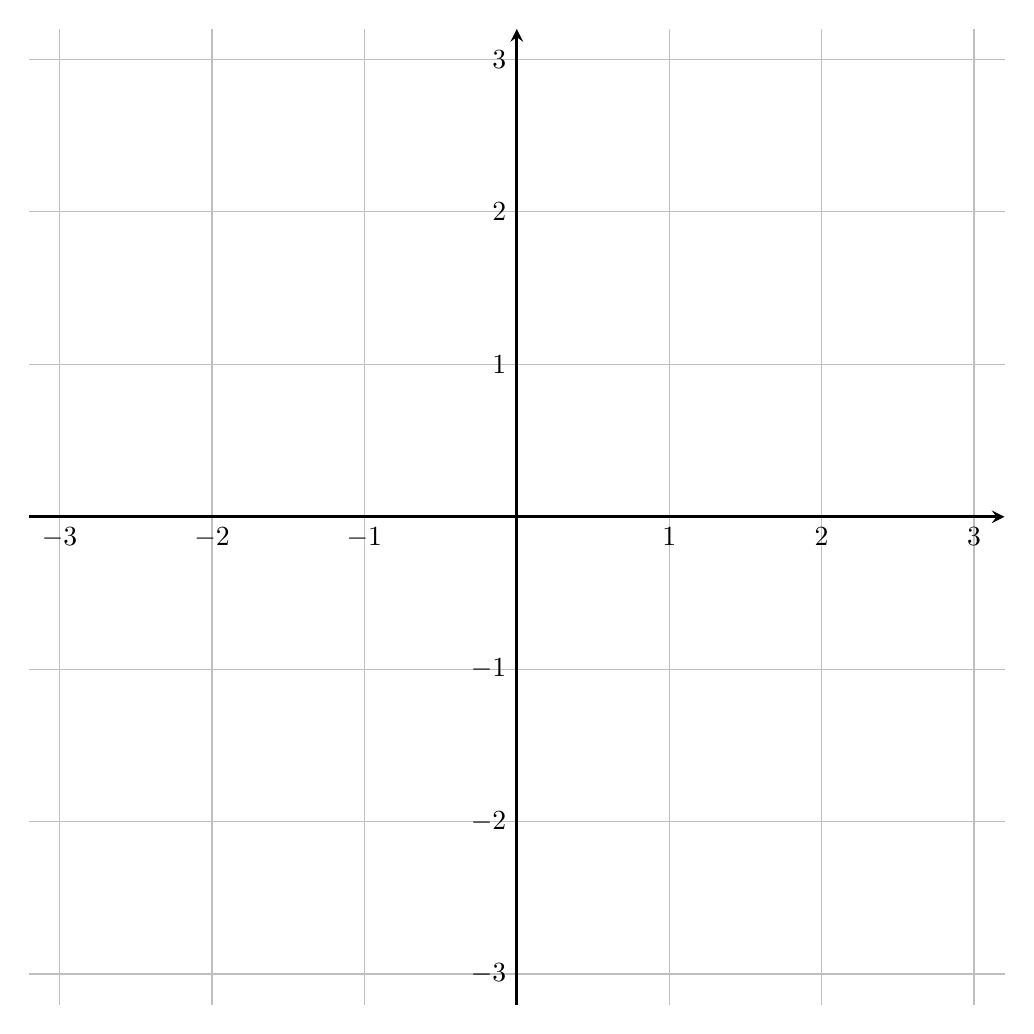
\begin{tikzpicture}
\begin{axis}[thick,smooth,no markers,
        xmin=-3.2, xmax=3.2,
        ymin=-3.2, ymax=3.2,
        xtick={-3,...,3},  
        % xticklabels= {,,},
        ytick={-3,...,3},
        % yticklabels= {,,},
        major tick length={0},
        line width=1pt,
        axis lines=center, height=5.5in, width = 5.5in, grid=major]
        % \addplot [domain=0.01:4.5, samples=100, name path=f, thick, color=red!50]
        % {sqrt(x)} node[above,pos=0.5] {$\sqrt{x}$} ;
        % \addplot [domain=0.4:4.5, samples=100, name path=g, thick, color=blue!50]
        % {x^(-2)} node[right,pos=0.5] {$\frac{1}{x^2}$} ;
        % \addplot[blue!50, opacity=0.3] fill between[of= f and g, soft clip={domain=1:4}];
\end{axis}
\end{tikzpicture}
\vspace{1.5in}
\end{center}

\pagebreak

\question $\ $

\begin{parts}
    \part[10]
    Show that the equation $3x + 2\cos{x} + 5 = 0$ has a root. State any theorems used and justify their use.
    \vfill
    \part
    (7 points \textbf{EXTRA CREDIT}) Show that the above equation has exactly one root. State any theorems used and justify their use.
    \vfill
\end{parts}

\pagebreak

\question[10] Find the point on the line $y=2x+3$ that is closest to the point $(0,0)$.
\vfill

\pagebreak

\question[10] Evaluate the following
\[\frac{d}{dx} \int_{2x}^{\pi/2} \sin{\frac{t}{2}}\cos{\frac{t}{3}} \ dt.\]
\vfill
\question Evaluate the following definite integrals, if they exist.
\begin{parts}
    \part[10] $\displaystyle \int_1^5 \frac{dt}{(t-4)^2}$
    \vfill
    \pagebreak
    \part[10] $\displaystyle \int_0^{\pi/4} (1+\tan{\theta})^3 \sec^2{x} \ dx$
    \vfill
    \part[10] $\displaystyle \int_{-\pi/4}^{\pi/4} x^4 \tan{x} \ dx$
    \vfill
\end{parts}

\pagebreak

\question[20] Find the volume of a solid obtained by rotating the region bounded by the given curve about the specified axis.
\begin{align*}
    & y = 2x \\
    & y = x^2\\
    & \text{About the $x$-axis}
\end{align*}
\end{questions}
\pagebreak
This page may be used as scratch paper

\pagebreak
This page may be used as scratch paper

\pagebreak
This page may be used as scratch paper
% \pagebreak

% \subsection*{Formula sheet}

% \begin{itemize}

% \item Derivatives of inverse trigonometric functions.

% \begin{align*}
% \frac{d}{dx} \sin^{-1}(x) & = \frac{1}{\sqrt{1-x^2}}~~~\text{(true for $-1<x<1$)} \\ \\
% \frac{d}{dx} \tan^{-1}(x) &=\frac{1}{1+x^2}~~~\text{(true for all $x$)} \\ \\ 
% \frac{d}{dx}\sec^{-1}(x) & =\frac{1}{|x|\sqrt{x^2-1}} ~~~\text{(true for $x<-1$ and $x>1$)}
% \end{align*}

% \vspace{.5cm}

% \item Pythagorean identities (true for all $x$ where the functions involved are defined).

% $$
% \sin^2(x)+\cos^2(x)=1,~~~\tan^2(x)+1=\sec^2(x),~~~1+\cot^2(x)=\csc^2(x).
% $$

% \vspace{.5cm}

% \item Reduction of power formulas / double angle formulas for sine and cosine (true for all $x$).

% $$
% \cos^2(x)=\frac{1}{2}(1+\cos(2x)),~~~\sin^2(x)=\frac{1}{2}(1-\cos(2x))
% $$

% \vspace{.5cm}

% \item Addition formulas for sine and cosine (true for all $x$ and $y$).
% \begin{align*}
% \sin(x)\sin(y) & =\frac{1}{2}\cos(x-y)-\frac{1}{2}\cos(x+y) \\ \\ 
% \cos(x)\cos(y) &=\frac{1}{2}\cos(x-y)+\frac{1}{2}\cos(x+y) \\ \\
% \sin(x)\cos(y) &=\frac{1}{2}\sin(x-y)+\frac{1}{2}\sin(x+y)
% \end{align*}

% \vspace{.5cm}

% \item Integrals of tangent and secant.
% \begin{align*}
% \int \tan(x)dx & =-\ln|\cos(x)|+C \\ \\
% \int \sec(x)dx & =\ln|\sec(x)+\tan(x)|+C.
% \end{align*}

% \end{itemize}


% \pagebreak

% \begin{itemize}
% \item Standard power series expansions (centered at $a=0$).
% \begin{align*}
% e^x & = \sum_{n=0}^\infty \frac{x^n}{n!}~~~~~ \text{ (valid for all $x$)}.\\ &\\ 
% \sin(x) & = \sum_{n=0}^\infty \frac{(-1)^nx^{2n+1}}{(2n+1)!} ~~~~~\text{ (valid for all $x$)}.\\ & \\
% \cos(x) & = \sum_{n=0}^\infty \frac{(-1)^nx^{2n}}{(2n)!} ~~~~~\text{ (valid for all $x$)}.\\&\\
% \ln(1+x) & =\sum_{n=1}^\infty \frac{(-1)^{n-1}x^n}{n}~~~~~\text{ (valid for $|x|<1$)}.\\&\\
% (1+x)^m & = \sum_{n=0}^\infty \frac{m(m-1)\cdots (m-n+1)}{n!}x^n~~~~~ \text{ (valid for $|x|<1$)}.
% \end{align*}
% \item Error estimate for approximations by Taylor polynomials.\\  Say $f(x)$ is a function with derivatives of all orders on an interval $[b,c]$, and $a$ is a point in $[b,c]$.  Say $P_N(x)$ is the $N^\text{th}$ Taylor polynomial for $f(x)$ centered at $a$, and $R_N(x)=f(x)-P_N(x)$ is the error when approximating $f(x)$ by $P_N(x)$.  Then for all $x$ in $[b,c]$
% $$
% |R_N(x)|\leq \frac{M_{N+1}|x-a|^{N+1}}{(N+1)!},
% $$
% where $M_{N+1}$ is the largest value taken by the $(N+1)^\text{st}$ derivative of $f(x)$ on $[b,c]$.
% \end{itemize}
    
\end{document}
